% ---------------------------
% ---- Собственный класс ----
% theorem - теорема
% definition - определение
% lemma - лемма
% corollary - следствие
% remark - замечание
% example - пример
% derivation - блок для выражений
% ---------------------------
\documentclass{tmcorreport}

% ------------------------
% Кодировка и языки
% ------------------------
\usepackage[utf8]{inputenc}
\usepackage[T2A]{fontenc}
\usepackage[english,russian]{babel}

% ------------------------
% Математика
% ------------------------
\usepackage{amsmath, amssymb, amsthm, mathtools}

% ------------------------
% Графика и рисунки
% ------------------------
\usepackage{graphicx}
\usepackage{float}
\usepackage{tikz}
\usepackage{pgfplots}
\pgfplotsset{compat=1.18}

\begin{document}

\section*{Функциональные требования}
\begin{enumerate}
    \item Создать, открыть, удалить доску.
    \item Добавить пользователя к доске, исключить пользователя из доски.
    \item Создать, удалить роль.
    \item Изменить права роли (добавить права, удалить права).
    \item Назначить роль пользователю, снять пользователя с роли.
    \item Создать, изменить, удалить колонку/ряд.
    \item Создать, изменить, удалить таск.
    \item Добавить субтаск к таску, изменить, удалить субтаск.
    \item Перенести таск из одной области в другую.
    \item Добавить тег к таску, убрать тег с таска.
    \item Назначить таск пользователю, роли.
    \item Просмотреть доски, участником которых является пользователь.
    \item Просмотреть задачи, назначенные пользователю.
\end{enumerate}

\section*{Главная страница}
\begin{description}
    \item Панель верхнего меню, боковое меню с вкладками: Мои доски, Мои задачи. По умолчанию выбрана вкладка Мои доски.
    \item На вкладке Мои доски: в теле страницы обозначены все доски пользователя. Для каждой доски обозначено, какие роли назначены пользователю на этой доске (если назначены).
    \item На вкладке Мои задачи: в теле страницы обозначены все задачи, назначенные пользователю.
\end{description}

\subsection*{Сценарий: Создание новой доски}
\begin{enumerate}
    \item Администратор создает новую доску на вкладке Мои доски $\to$ Новая доска.
    \item Новая доска создается на отдельной странице. Администратор вводит название доски, описание (опционально), добавляет зарегистрированных пользователей к доске (по логину/email; опционально).
    \item После создания доски открывается страница этой доски. По умолчанию в любой новой доске присутствуют три колонки: To-Do, In Progress, Done, и один неименованный ряд.
    \item Новые колонки и ряды могут быть добавлены нажатием кнопки в правой части заголовков колонок и в нижней части названий рядов соответственно.
    \item Администратор создает таск в любой области двойным нажатием. Таск добавляется в выбранную область (пересечение колонки и ряда).
    \item Роли могут быть созданы в настройках доски. Добавление пользователей к доске происходит также через настройки доски.
\end{enumerate}

\subsection*{Сценарий: Создание колонки (ряда)}
\begin{enumerate}
    \item Название колонки (ряда) вводится на доске при создании (или нажатии на него).
    \item Администратор может назначить колонке (ряду) статус готовых тасков в настройках колонки (ряда). Статус подразумевает что таски, добавленные в эту колонку, будут автоматически помечены, как завершенные. При переносе тасков в другие колонки, не имеющими статус, статус завершенные с них снимается.
    \item Администратор может назначить различные права доступа к колонке (ряду) различным пользователям (ролям) в настройках колонки (ряда). Права доступа: просмотр колонки (ряда), создание тасков, перенос тасков (из и в колонку).
\end{enumerate}

\subsection*{Сценарий: Создание таска}
\begin{enumerate}
    \item На доске создается таск, пользователь вводит его название.
    \item Администратор может перейти в настройки таска нажатием на него. В показывающейся панели пользователь может ввести описание таска, назначить его пользователям (ролям), добавить теги, пометить таск как выполненный.
    \item Субтаски добавляются к таску на доске или в настройках. Субтаски обладают тем же поведением и характеристиками, что и таски, но не могут быть отделены от родительского таска.
\end{enumerate}

\section{Ролевая модель}
Каждая доска имеет две роли по умолчанию: \textbf{Пользователь} и \textbf{Администратор}. Права пользователя для каждой доски может определять \textbf{Администратор}, однако удалять эту роль \textbf{Администратор} не может. 

По умолчанию права \textbf{Пользователя:}
\begin{itemize}
    \item добавление тасков к любым колонкам (рядам);
    \item добавление субтасков к созданным им или назначенных ему таскам;
    \item изменение статуса созданных им или назначенных ему тасков/субтасков;
    \item перенос созданных им или назначенных ему тасков;
\end{itemize}
\textbf{Администратор} обладает всеми правами и не может изменить права \textbf{Администратора}.\\\\
\textbf{Администратор} может создавать новые Роли и назначать им следующие права:
\begin{itemize}
    \item добавление тасков к любым колонкам (рядам) (ограничения на конкретные колонки (ряды) накладываются в настройках соответствующих колонок (рядов));
    \item добавление субтасков к любым таскам, только к созданным самим, пользователем, только к назначенным пользователю, к созданным и к назначенным;
    \item изменение статусов любых тасков (субтасков), только к созданным самим пользователем, только к назначенным пользователю, к созданным и к назначенным;
    \item создание и удаление новых колонок (рядов);
    \item изменение доступа к колонкам (рядам);
    \item назначение тасков пользователям;
    \item изменение, удаление любых тасков, только назначенных пользователю;
\end{itemize}
\section{Статусная модель}
Только два стасуса: закончен таск или нет. Таск может быть помечен как законченный вручную, или автоматически при переносе в колонку (ряд), помеченную как колонку для законченных тасков. Законченный статус может быть снят.

\section{Модель данных}
\begin{figure}[H]
    \centering
    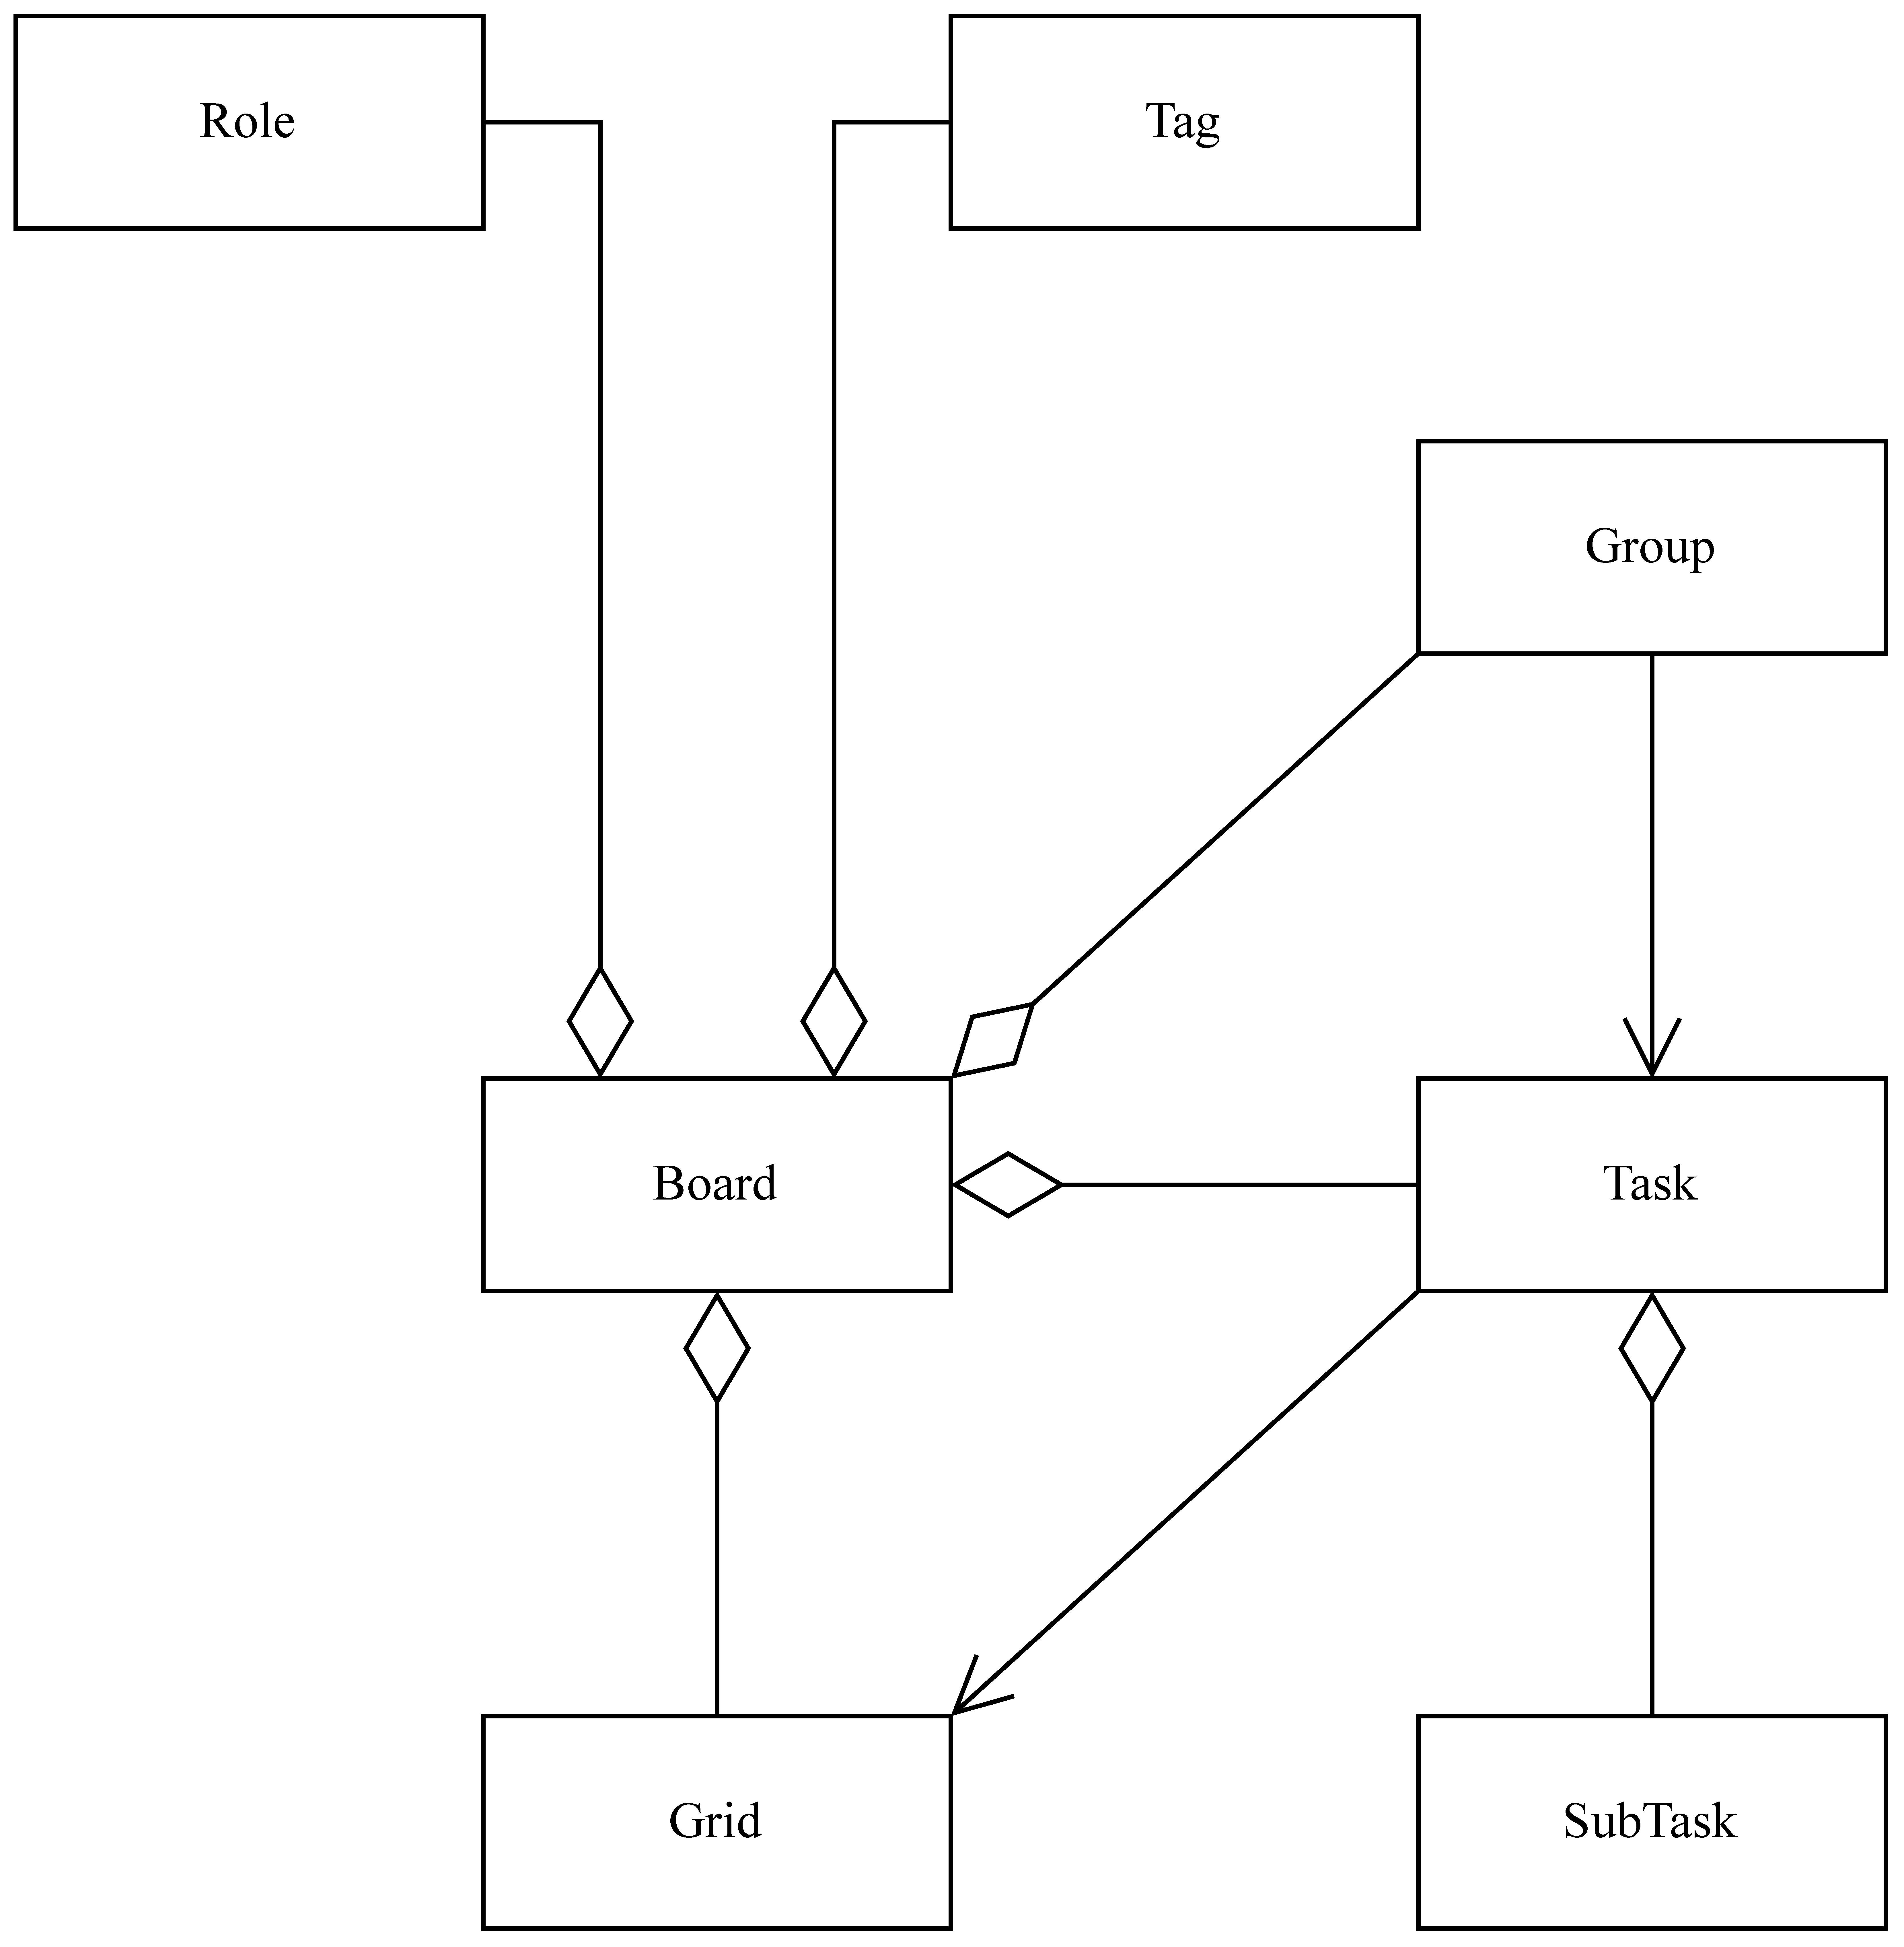
\includegraphics[width=0.55\textwidth]{img/DC.pdf}
\end{figure}
\begin{itemize}
    \item \textbf{Board} -- Контейнер для всей структуры: хранит колонки/дорожки (\textbf{Grid}), таски, теги и настройки доступа.
    \item \textbf{Role} - Определяет права пользователей на доске.
    \item \textbf{Tag} - Короткая метка для классификации тасков и субтасков.
    \item \textbf{Group} - Объединение связанных тасков по какому-либо признаку (например, эпик, модуль, категория таски).
    \item \textbf{Task} - Основная рабочая единица: таска с описанием, статусом, тегами, группой и подзадачами.
    \item \textbf{Grid} - дорожка/столбец. Структурный элемент доски, в котором размещаются таски.
    \item \textbf{SubTask} - Часть задачи, вложенная в таск, используемая для дробления работы.
\end{itemize}
\section{Обработки исключений}
\begin{enumerate}
    \item \textbf{Перенос таски с незаконченными субтасками} в колонку (ряд) завершенных тасков - должно показываться предупреждение, что все субтаски при переносе также будут отмечены, как завершенные.
    \item \textbf{Противоречивость прав} - например, пользователю запрещен просмотр некоторой колонки, однако ему назначена роль, которая имеет к колонке полный доступ. Решение: приоритет прав пользователей над правами ролей.
    При назначении пользователю ролей с противоречивыми правами используется высший уровень прав среди назначенных.
    \item \textbf{При попытке пользователя перейти к доскам}, таскам, к которым он не имеет доступа (например, по URL), отображать страницу (или сообщение) с сообщением о недостаточных правах.
    \item \textbf{Валидация текстовых полей на инъекцию кода}.
\end{enumerate}

\end{document}